\documentclass[a4paper,oneside,bibtotoc,smallheadings,pointlessnumbers,
halfparskip,DIV15]{scrartcl}
% kate: remove-trailing-space on; replace-trailing-space-save on; indent-width 2; indent-mode normal; space-indent on;
% tocleft,
\usepackage[pdftex]{graphicx}
\usepackage[ngerman]{babel}
\usepackage[utf8]{inputenc}
\usepackage{../../assets/uniinput}
\usepackage[T1]{fontenc}
\usepackage{amssymb,amsmath}
\usepackage{booktabs}
\usepackage{enumerate}
\usepackage{subfig}
% \usepackage{siunitx}
% \sisetup{
%   seperr         = true,
%   trapambigerr   = true,
%   openerr        = (,
%   closeerr       = ),
%   expproduct     = cdot,
%   padnumber      = both,
%   stickyper      = true,
%   per            = reciprocal,
%   trapambigfrac  = true,
%   repeatunits    = false,
%   openfrac       = (,
%   closefrac      = ),
%   prefixsymbolic = true,
%   prefixproduct  = cdot,
%   decimalsymbol  = comma,
%   tabnumalign    = left,
%   tabtextalign   = left
% }
\usepackage{color}
\definecolor{grey}{rgb}{.4,.4,.4}
\definecolor{darkgreen}{rgb}{0,.35,0}
\definecolor{ltgray}{gray}{0.95}
% \definecolor{darkblue}{rgb}{0,0,.6}
% \definecolor{darkred}{rgb}{.6,0,0}
% \definecolor{red}{rgb}{.98,0,0}
\usepackage{listings}
\lstdefinelanguage{Maxima}{
  keywords={addrow,addcol,zeromatrix,ident,augcoefmatrix,ratsubst,diff,ev,tex,%
    with_stdout,nouns,express,depends,load,submatrix,div,grad,curl,%
    rootscontract,solve,part,assume,sqrt,integrate,abs,inf,exp,float,log},
  sensitive=true,
  comment=[n][\itshape]{/*}{*/}
}
\lstdefinelanguage{C++}{
%   commentstyle=\itshape\color{darkgreen},
%   commentstyle=\color{darkgreen},
%   keywordstyle=\bfseries, %\color{darkblue},
%   stringstyle=\color{darkred},
%   basicstyle=\ttfamily\scriptsize,
  morekeywords={TH1F,TLorentzVector,TVector3,vector,TFile,TFitResultPtr,TF1,\
                TGraph,TH1,TObject,TCanvas,string,Double_t,TGraphErrors},
  basicstyle=\scriptsize,
  numbers=left,
  numberstyle=\tiny,%\color{gray},
  stepnumber=1,
  tabsize=4,
  showspaces=false,
  showstringspaces=false,
  breaklines=true,
  frame=lrtb,
  captionpos=b,
  extendedchars=true,
  inputencoding=utf8,
%   backgroundcolor=\color{ltgray}
}
% \usepackage{courier}
\lstset{language=Matlab,
%     keywords={break,case,catch,continue,else,elseif,end,for,function,global,if,otherwise,persistent,return,switch,try,while},
%     basicstyle=\ttfamily\small,%\scriptsize,
  basicstyle=\scriptsize,
  keywordstyle=\bfseries,
  commentstyle=\itshape\color{blue},
  stringstyle=\itshape,
  identifierstyle=\ttfamily,
  numbers=left,
  numberstyle=\tiny,
  stepnumber=1,
  tabsize=2,
  showspaces=false,
  showstringspaces=false,
  breaklines=true,
  frame=single,
  columns=fixed,
  captionpos=b,
  extendedchars=\true,
  inputencoding=utf8,
  backgroundcolor=\color{ltgray},
  postbreak = \raisebox{0ex}[0ex][0ex]{\ensuremath{\hookrightarrow}}
%   linewidth=0.9\textwidth
}
\usepackage[pdftex]{hyperref}
\hypersetup{
%   colorlinks  = true,
%   urlcolor    = darkblue,
  pdftitle    = {Protokoll zum CPII-Übungsblatt 4},
  pdfsubject  = {Protokoll Computational Physics}
  pdfauthor   = {robert.riemann@physik.hu-berlin.de,thomas.murach@physik.hu-berlin.de},
%   pdfkeywords = {Computational Physics,CP,II,2010,Jacobi-Methode,Diagonalisierung,Eigenwerte, Eigenvektoren,eig,octave,matlab}
%   pdfcreator  = {pdftex},
%   pdfproducer = {pdftex}
}

\newcommand{\dd}[1]{\mathrm{d}#1\,} % declare dx operator, usage: \dd{x} for dx
\newcommand{\lref}[1]{Listing~(\ref{lst:#1})} % refer to a listing, usage: \lref{label} for Listing (...)
\newcommand{\fref}[1]{Abb.~(\ref{fig:#1})} % refer to a figure, usage: \lref{label} for Abb. (...)
\newcommand{\tref}[1]{Tab.~(\ref{tab:#1})} % refer to a table, usage: \lref{label} for Tab. (...)
\newcommand{\eref}[1]{Gl.~(\ref{eqn:#1})} % refer to a equation, usage: \lref{label} for Tab. (...)

\begin{document}
% % % % % % % % % % % % % % % % % % % % % % % %
\title{{\centering \rule{15cm}{0.001cm}\\
\Large{\textsc{Institut für Physik der
Humboldt-Universität zu Berlin}}}\\ \centering \rule{15cm}{0.001cm}\\
\vspace{15mm} \centering
\includegraphics[scale=0.9]{../../assets/siegel}\\
\vspace{18mm}
{\bf{\huge{Computational Physics II}}}\\
\vspace{12mm}
Übungsblatt 4\\
\vspace{15mm}
% Compton-Effekt\\
% \vspace{14mm} {\small{\textbf{Betreuer: M. zur Nedden}}}\\}
}
\author{Robert Riemann; Matr.Nr.: 521085\\
Thomas Murach; Matr.Nr.: 517771\vspace{18mm}}
% \vspace{8mm}
% \date{15. Juni 2008}
% % % % % % % % % % % % % % % % % % % % % % % %
% \onecolumn
\maketitle
% \twocolumn

\newpage
% \tableofcontents
% \listoffigures
% \listoftables
\section*{Aufgabe 1}
\subsection*{1a)}
Zunächst soll der Ausdruck für die eindimensionale Zustandssumme $Z$ für das
Ising-Modell (Hamiltonian s. Skript) mit nicht verschwindendem Magnetfeld hergeleitet werden. Diese ist
nach dem Skript, Gl. (8.14), zu bestimmen als
\begin{eqnarray}
Z &=& \mathrm{Tr}\left[T^L\right]\\
\mathrm{mit\quad} T_{σσ'} &=& \exp[βσσ' + βB(σ+σ')/2]
\end{eqnarray}
σ und $σ'$ können hierbei $\pm 1$ sein. Damit ergibt sich die folgende Matrix $T$:
\begin{eqnarray}
T = \begin{pmatrix} e^{β(1+B)} & e^{-β} \\ e^{-β} & e^{β(1-B)} \end{pmatrix}
\end{eqnarray}

Nun sind die Eigenwerte dieser Matrix zu berechnen, um eine Diagonalform herstellen zu können,
mit dem Ziel, die Potenzierung der Matrix möglichst einfach werden zu lassen. Dies wird in den folgenden
Zeilen getan.

\begin{eqnarray}
0 &=& \det[T-λ] = (e^{β(1+B)}-λ)(e^{β(1-B)}-λ) - e^{-2β}\\
&=& λ^2 - λe^β\underbrace{\left(e^{βB} + e^{-βB}\right)}_{2\cosh(βB)} + \underbrace{e^{2β} - e^{-2β}}_{2\sinh(2β)}\\
→ λ_{\pm} &=& e^β\cosh(βB) \pm \sqrt{e^{2β}\cosh^2(βB) - 2\sinh(2β)}
\end{eqnarray}

Damit lässt sich die Potenzierung und anschließende Spurbildung der Matrix leicht
analytisch durchführen:
\begin{eqnarray}
\mathrm{Tr}[T^L] = λ_+^L + λ_-^L
\end{eqnarray}

$Z$ ist somit exakt bekannt. Um nun den Grenzwert $L→∞$ durchzuführen, wird ausgenutzt,
dass $λ_-$ kleiner als $λ_+$ ist. Daher ist der Beitrag von $λ_-$ im Grenzfall
vernachlässigbar.

\begin{eqnarray}
Z \approx λ_+^L = \left(e^β\cosh(βB) + \sqrt{e^{2β}\cosh^2(βB) - 2\sinh(2β)}\right)^L
\end{eqnarray}

\subsection*{1b)}
Hier soll aus der bekannten, kanonischen Zustandssumme die mittlere Energie und
Magnetisierung berechnet werden. Dafür wird die Relation aus Skript, Gl. (8.9) (mittlere
Energie) und Gl. (8.10) (mittlere Magnetisierung) verwendet. Die Relation für die mittlere
Energie $E$ lautet wie folgt:
\begin{eqnarray}
E &=& \langle H \rangle = -\frac{∂\ln Z}{∂β}\\
&=& {{\left({{2e^{2β}B\cosh \left(βB\right)\sinh \left(βB\right)+2e^{2β}\cosh^2
 \left(βB\right)-4\cosh \left(2β\right)}\over{2\sqrt{
 e^{2β}\cosh ^2\left(βB\right)-2\sinh \left(2β\right)}}}+e^β(B\sinh \left(βB\right)+
 \cosh \left(βB\right))\right)L}
 \over{\sqrt{e^{2β} \cosh^2\left(βB\right)-2\sinh \left(2β\right)}+e^{
 β}\cosh \left(βB\right)}}
\end{eqnarray}

Für die Magnetisierung $M$ ergibt sich folgendes:
\begin{eqnarray}
\langle M \rangle &=& \frac{1}{β}\frac{∂\ln Z}{∂B}\\
&=& {L\left({{e^{2β}\cosh \left(βB\right)\sinh \left(βB\right)}\over{\sqrt{e^{2β}\cosh^2
 \left(βB\right)-2\sinh \left(2β\right)}}}+e^β \sinh \left(βB\right)\right)}
 \over{\sqrt{e^{2β}\cosh ^2\left(βB\right)-2\sinh \left(2β\right)}+e^{β}\cosh \left(βB\right)}
\end{eqnarray}

\subsection*{1c}

Schließlich war die Magnetisierung in Abhängigkeit von β und $B$ zu plotten.
Dafür wurde das in \lref{plot_mag} dargestellte Skript geschrieben.

\lstinputlisting[label=lst:plot_mag,caption={magnetisierung.m}]{../code/magnetisierung.m}

Die daraus erstellte Graphik ist in \fref{magnetisierung} dargestellt.

\begin{figure}[htb]
  \centering
  \includegraphics[width=0.8\columnwidth,keepaspectratio]{../tmp/magnetisierung-crop}
  \caption{Magnetisierung in Abhängigkeit von β und $B$, jeweils in natürlichen Einheiten}
  \label{fig:magnetisierung}
\end{figure}

Das Ergebnis entspricht den Erwartungen, da bei großen Magnetfeldern die Magnetisierung
ihren positiven oder negativen Grenzwert anstrebt, je nach Ausrichtung des Magnetfelds.
Weiterhin ist zu beobachten, dass bei kleinen Temperaturen, also großen β-Werten,
die Magnetisierung fast sofort ihren Grenzwert erreicht, während bei großen Temperaturen,
also kleinen β-Werten, auch große äußere Magnetfelder die Magnetisierung nicht 
wesentlich vom Wert $M=0$ abweichen lassen. Dies entspricht der Vorstellung, dass
eine hohe Temperatur die einzelnen Spins stärker aus der Ausrichtung in eine
Richtung ablenkt als eine geringe Temperatur.

\section*{Aufgabe 2)}

In der zweiten Aufgabe wurde ein ein- und ein zweidimensionales Spin-Gitter untersucht.
Dabei sollten diese Gitter jeweils einmal geordnet und einmal ungeordnet, also
zufällig belegt sein. Für alle Fälle war die Magnetisierung und die Energie zu messen.
Die Randbedingungen waren periodisch.

Der Code, der diese Aufgabenstellung bearbeitet, ist in \lref{main} dargestellt.

\lstinputlisting[label=lst:main,caption={main.cpp}]{../code/main.cpp}

Als Zufallszahlengenerator wurde die in der ROOT-Klasse \texttt{TRandom3} zur
Verfügung gestellte Funktion \texttt{Uniform} verwendet, die gleichverteilte Zufallszahlen
generiert.

Weiterhin wurde immer überprüft, welche Indizes die Nachbarn des Koordinatenursprungs haben,
um die korrekte Implementierung der Randbedingungen zu testen.

Das Programm wurde mit verschiedenen Parametern aufgerufen, um die einzelnen
Konfigurationen zu testen, wobei der folgende Output resultierte:

\begin{lstlisting}[caption=Aufruf und Output von \lref{main},label=lst:output]
$> ./main 10 1 0
magnetization: 0.4
energy: 10
neighbours of (0,0,...):
  1
  9
$> ./main 10 1 1
magnetization: 1
energy: 40
neighbours of (0,0,...):
  1
  9
$> ./main 10 2 0
magnetization: 0.46
energy: 176
neighbours of (0,0,...):
  1
  10
  9
  90
$> ./main 10 2 1
magnetization: 1
energy: 600
neighbours of (0,0,...):
  1
  10
  9
  90
\end{lstlisting}
Unabhängig von der Dimension ist demnach die Energie und die Magnetisierung für
geordnete Systeme deutlich größer als für ungeordnete Systeme, was zu erwarten
war. Auch die Überprüfung der Nachbarn stimmt mit den Erwartungen überein. 
% \section*{3.1b)}

Zu zeigen ist der Zusammenhang, der zwischen der logistischen Abbildung mit $r = 4$
\begin{equation}
 M_L(x_n) = 4x_n(1-x_n) = x_{n+1}
 \label{eqn:ml}
\end{equation}
und der Dreiecksabbildung
\begin{equation}
 \label{eqn:md}
 M_D(x_n) = \left(1-2\left|\frac{1}{2}-x\right|\right) = x_{n+1}
\end{equation}
besteht.

Nun substituieren wir $x_n$ in \eref{ml} mit:
\begin{equation}
 x_n = \sin^2\left(\frac{\pi}{2}\alpha_n\right)
\end{equation}
Hierbei wird darauf geachtet, dass die Substitution selbst auch eine Abbildung
von $[0, 1]$ nach $[0, 1]$ darstellt. Man erhält:
\begin{eqnarray}
 M_L(x_n) = x_{n+1} &=& 4x_n(1-x_n) \\
 \sin^2\left(\frac{\pi}{2}\alpha_{n+1}\right) &=& 4\sin^2\left(\frac{\pi}{2}\alpha_n\right)\underbrace{\left(1-\sin^2\left[\frac{\pi}{2}\alpha_n\right]\right)}_{\cos^2\left(\frac{\pi}{2}\alpha_n\right)} \\
 &=& 4\left[ \sin\left(\frac{\pi}{2}\alpha_n\right)\cos\left(\frac{\pi}{2}\alpha_n\right)\right]^2 = 4 \left[ \frac{1}{2} \sin\left( 2 \frac{\pi}{2} \alpha_n \right) \right]^2 = \sin^2\left(\frac{\pi}{2}2\alpha_n\right) \\
 \rightarrow \alpha_{n+1} &=& \pm 2 \alpha_n
\end{eqnarray}

Wie aus der Vorlesung bekannt ist, hat die logistische Abbildung ebenfalls eine
Stretching-Wirkung mit Faktor 2. Das Vorzeichen hängt hierbei von $x$ ab und ist
für Werte $\in [0; 0.5]$ positiv.

Darauf folgt die Equivalenz des invarianten Maßes der Dreiecksabbildung $ρ_D = 1$
und der logistischen Abbildung in Abhängigkeit von $alpha$ $ρ_L(α)$:
\begin{equation}
 ρ_D = ρ_L(α) = 1 
\end{equation}
Es gilt weiterhin:
\begin{eqnarray}
 ρ_L(α)\dd{α} &=& ρ_L(x)\dd{x} \\
  \rightarrow ρ_L(x) &=& \underbrace{ρ_L(α)}_{=1} \frac{\dd{\alpha}}{\dd{x}} \\
 \frac{\dd{x}}{\dd{α}} &=&  π \sin\left(\frac{\pi}{2}\alpha\right)\cos\left(\frac{\pi}{2}\alpha\right) = π\sqrt{x(1-x)} \\
 \rightarrow ρ_L(x) &=& \frac{1}{\pi\sqrt{x(1-x)}}
\end{eqnarray}

Der Vergleich zwischen experimentellem und theoretischem Ergebnis ist in \fref{1b}
veranschaulicht. Die rote Line beschreibt den auf die experimentellen Daten
renormierten theroretischen Verlauf $ρ_L(x)$.
\begin{figure}[htb]
\centering
  \includegraphics[width=1\columnwidth,keepaspectratio]{../logabb_r4.png}
  \caption{Vergleich zwischen Experiment und Theorie von $ρ_L(x)$}
  \label{fig:1b}
\end{figure}






\section*{Aufgabe 2a)}

Der Bearbeitung der Aufgabe 2 liegt die Funktion \texttt{homo\_ocs.m} zu Grunde,
welche den Hamilton-Operator mit Potential in Abhängigkeit von α in Matrix-Darstellung
zurück gibt. Sie ist in \lref{2funk} abgedruck.

\lstinputlisting[label=lst:2funk,caption={homo\_ocs.m}]{../code/homo_osc.m}

Zunächst sollten für verschiedene α die drei niedrigsten Eigenwerte bestimmt werden.
Der Quellcode ist hierfür in \lref{2a} zu finden.
\lstinputlisting[firstline=64,lastline=70,label=lst:2a,caption={steuerung.m}]{../code/steuerung.m}

\begin{lstlisting}[caption=Ausgabe von \lref{2a},label=2aa]
eigen_values =
    alpha=1   alpha=2   alpha=3   alpha=4
    0.5087    0.5000    0.5115    0.5302
    1.1691    1.5000    1.7253    1.8998
    1.6239    2.5000    3.1851    3.7278
\end{lstlisting}

In der Ausgabe \lref{2aa} sind die Ergebnisse dargestellt. Die 3 niedrigsten Eigenwerte
für ein α befinden sich jeweils in einer Spalte. Man kann sehr gut erkennen, dass man für
$α = 2$ das analytische Ergebniss erhält. Ein Vergleich mit den Daten aus CP1 ist
weiterhin nicht sinnvoll, da das Potential anders definiert war. Für den Spezialfall
$α = 2$ deckt sich zufällig das damals definierte Potential mit dem in für diese
Übung verwendeten. Das Ergebnis für die Eigenwerte lautete damals:
\begin{equation*}
0.500000,\;1.500000,\;2.499999
\end{equation*}
Beim Vergleich stellen wir als fest, dass die in dieser Übung verwendete Methode
zur Bestimmung der Eigenwerte genauer ist. Damals wurde eine Differentialgleichung
mit dem Runge-Kutta-Verfahren gelöst.



\section*{Aufgabe 2b)}

Der Quellcode für diese Teilaufgabe ist in \lref{2b} gegeben.
\lstinputlisting[firstline=74,lastline=93,label=lst:2b,caption={steuerung.m}]{../code/steuerung.m}

Um zu zeigen, dass der Fehler exponentiell abnimmt, wenn $N$ linear vergrößert
wird, wurde die relative Abweichung vom Mittelwert der 4 Eigenwerte mit den jeweils
größten $N$ geplottet. Das Ergebnis ist in \fref{62b} dargestellt. Man erkennt,
dass der Fehler tatsächlich exponentiell abfällt (im Log-Plot linear) und bei
 $N > 75$ schließlich konstant bleibt. Die untere Grenze für den relativen Fehler
ergibt sich aus der endlichen Maschinengenauigkeit.

\begin{figure}[htb]
  \centering
  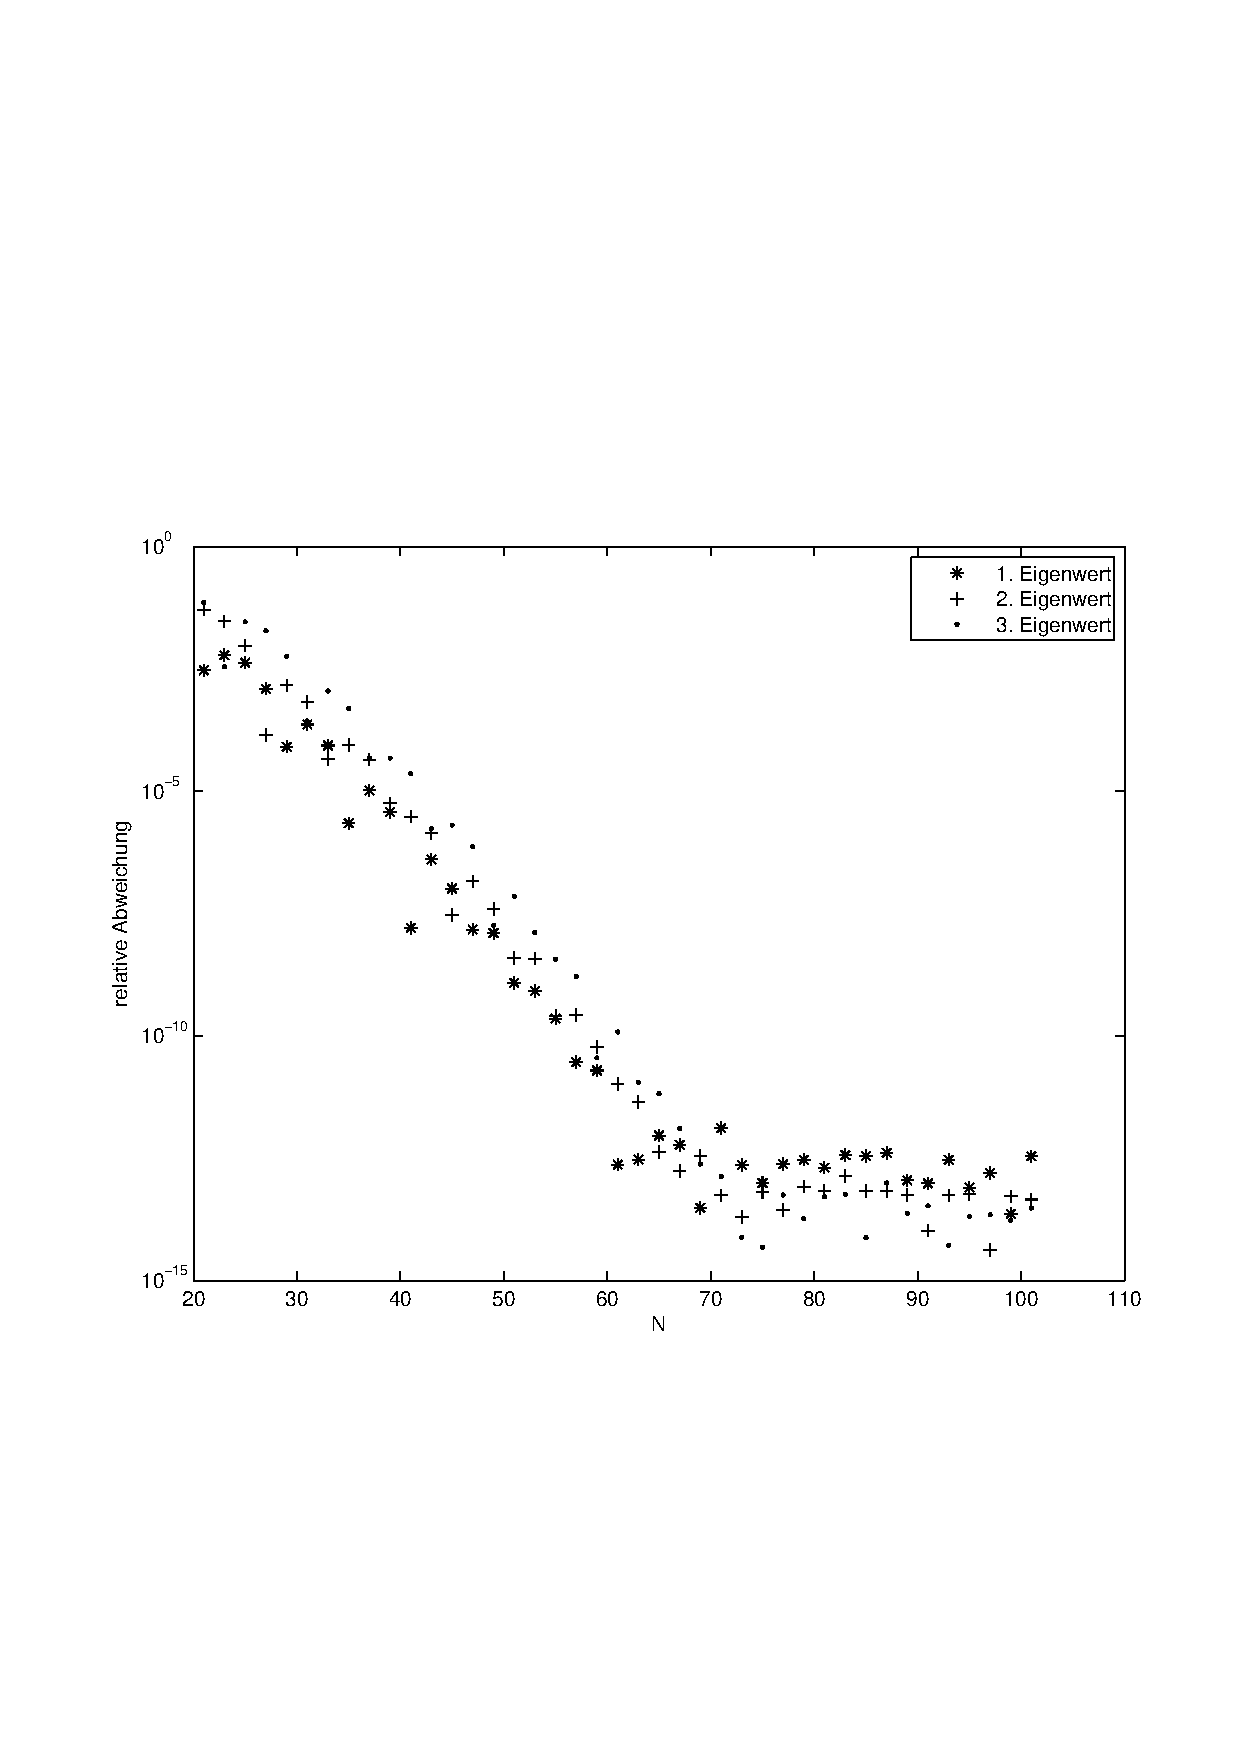
\includegraphics[width=0.8\columnwidth,keepaspectratio]{../tmp/plot62b.png}
  \caption{Halblogarthmischer Plot zur Abhängigkeit des Fehlers von der Diskretisierung.}
  \label{fig:62b}
\end{figure}
% \input{auswertung}
% \input{ergebnis}
% \input{quellen}
% \input{anhang}

% \section{Beispiele}
% blabla
%
% Weitere Information sind der Versuchsbeschreibung im \cite{script} zu entnehmen.
%
% \lstinputlisting[firstline=2,firstnumber=1,label=lst:aufruf,caption={aufruf.m - Matlab Batchdatei}]{aufruf.m}
%
% \begin{eqnarray}
% 	g &=& \SI{9.8157(11)}{\metre\per\second\squared} \\
%         \left[ g \right] &=& \si{\metre\per\Square\second} % großschreibung!
% 	\label{eqn:asdf}
% \end{eqnarray}
%
% Dann kann man auf \eref{asdf} verweisen.


% \begin{figure}[htb]
% 	\centering
% 	\includegraphics[width=1\columnwidth,keepaspectratio]{Winkelabhaengigkeit2}
% 	\caption{Periodendauer in Abhängigkeit der Maximalauslenkung}
% 	\label{fig:Winkelabhaengigkeit}
% \end{figure}

% \begin{table}[htbp]
% \centering
% \setlength{\tabcolsep}{14pt}
% \begin{tabular*}{\columnwidth}{%
% S[tabformat=2.1]%
% S[tabformat=2.2]%
% S[tabformat=1.2]}
% \toprule
% {$R$ in \si{\ohm}} &
% {$U$ in \si{\volt}} &
% {$\frac{U}{U_{R=0}}$}\\
% \midrule
% \multicolumn{3}{c}{\textit{Eingangswiderstand $R_E$}}\\
% \midrule
% 0 & 16 & 1 \\
% 4.7e3 & 8 & 0.5 \\
% \midrule
% \multicolumn{3}{c}{\textit{Ausgangswiderstand $R_A$}}\\
% \midrule
% 0 & 1.8 & 1 \\
% 12 & 0.52 & 0.29 \\
% 27 & 1.2 & 0.67 \\
% 18 & 0.8 & 0.44 \\
% \bottomrule
% \end{tabular*}
% \label{tab:221messungexp_widerstaende}
% \caption{experimentelle Messung der Ein- und Ausgangswiderstände}
% \end{table}


% \newpage

% \onecolumn
% \appendix
% \begin{figure}
% 	\centering
% 	\includegraphics[width=0.98\textwidth,keepaspectratio]{Messprotokoll}
% 	\caption{Messprotokoll}
% 	\label{fig:protokoll}
% \end{figure}
%\colorbox{yellow}{} Farben verwenden
\end{document}
